\section{HDF5 File}
\usetikzlibrary{trees}
\tikzstyle{every node}=[draw=black,thick,anchor=west]
\tikzstyle{dataset}=[fill=gray!30]
\tikzstyle{attribute}=[dashed,fill=gray!30]
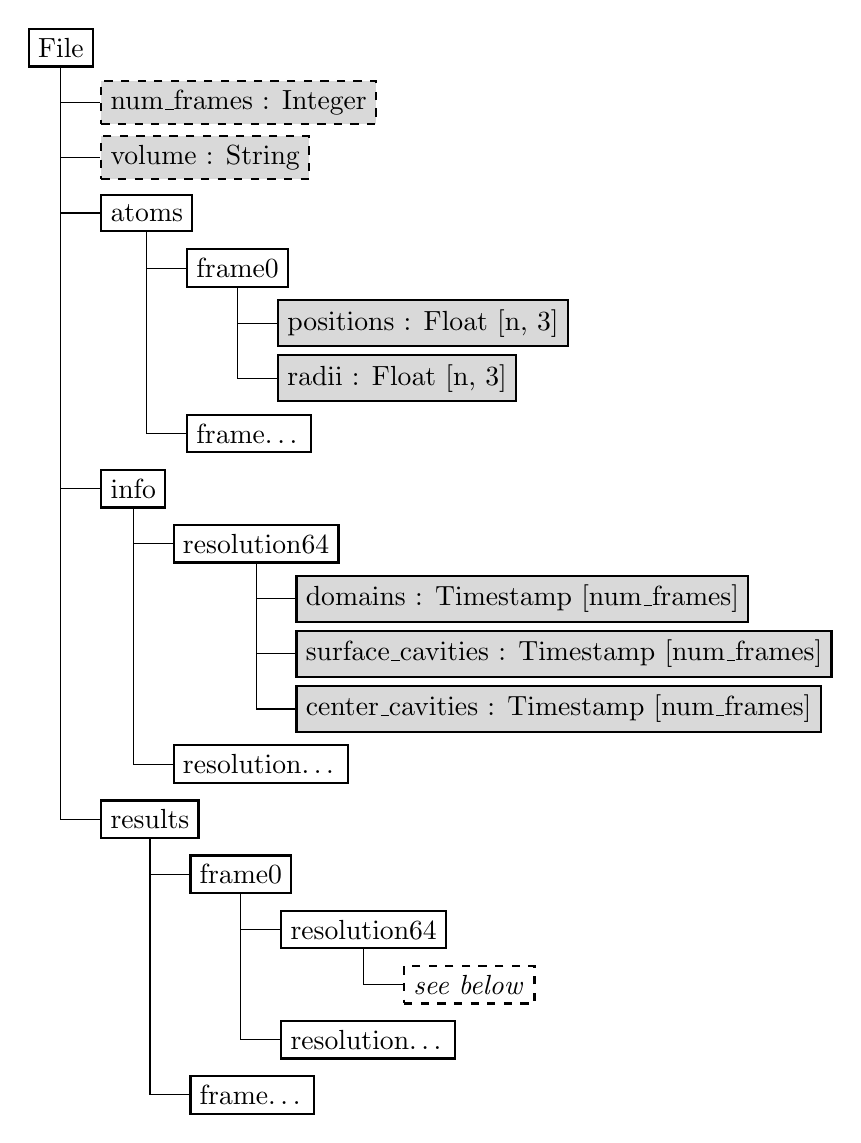
\begin{tikzpicture}[%
        grow via three points={one child at (0.5,-0.7) and
        two children at (0.5,-0.7) and (0.5,-1.4)},
        edge from parent path={(\tikzparentnode.south) |- (\tikzchildnode.west)}]
    \node{File}
    child{node[attribute]{num\_frames : Integer}}
    child{node[attribute]{volume : String}}
    child{node{atoms}
        child{node{frame0}
            child{node[dataset]{positions : Float [n, 3]}}
            child{node[dataset]{radii : Float [n, 3]}}
        }
        child[missing]{}
        child[missing]{}
        child{node{frame\ldots}}
    }
    child[missing]{}
    child[missing]{}
    child[missing]{}
    child[missing]{}
    child{node{info}
        child{node{resolution64}
            child{node[dataset]{domains : Timestamp [num\_frames]}}
            child{node[dataset]{surface\_cavities : Timestamp [num\_frames]}}
            child{node[dataset]{center\_cavities : Timestamp [num\_frames]}}
        }
        child[missing]{}
        child[missing]{}
        child[missing]{}
        child{node{resolution\ldots}}
    }
    child[missing]{}
    child[missing]{}
    child[missing]{}
    child[missing]{}
    child[missing]{}
    child{node{results}
        child{node{frame0}
            child{node{resolution64}
                child{node[dashed]{\textit{see below}}}
            }
            child[missing]{}
            child{node{resolution\ldots}}
        }
        child[missing]{}
        child[missing]{}
        child[missing]{}
        child{node{frame\ldots}}
    }
    child[missing]{}
    child[missing]{}
    child[missing]{}
    child[missing]{}
    child[missing]{}
    ;
\end{tikzpicture}

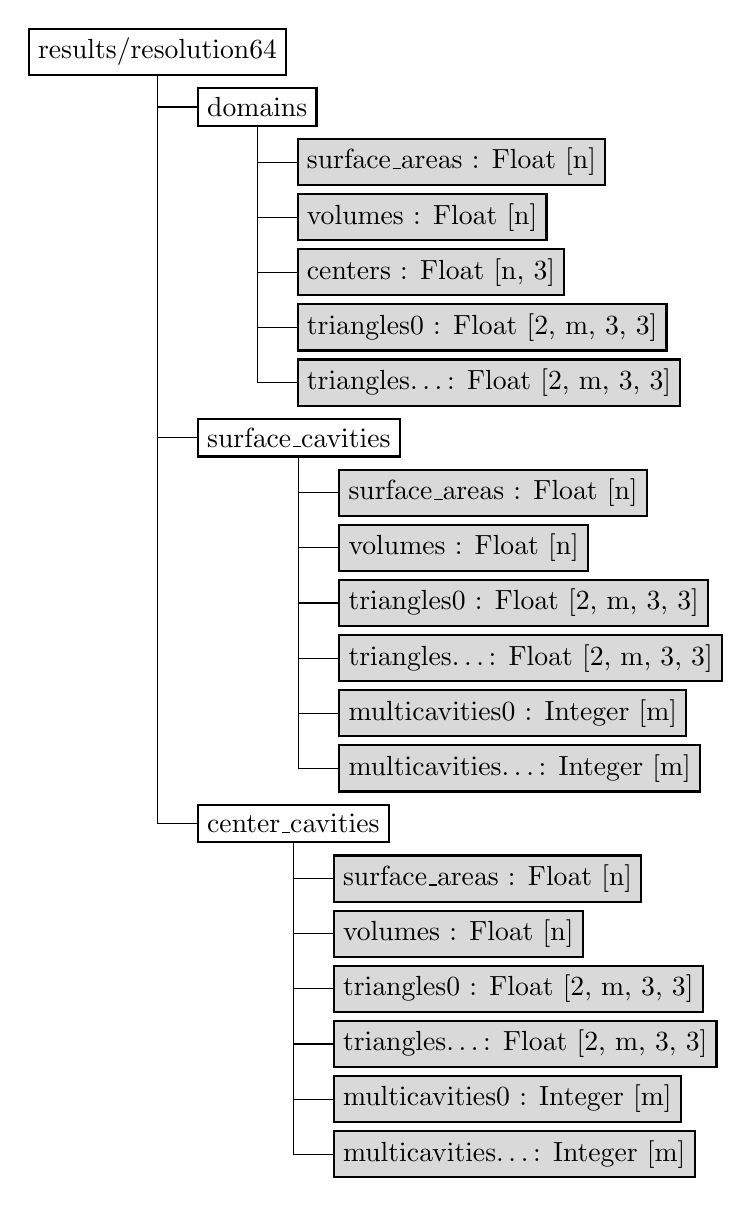
\begin{tikzpicture}[%
        grow via three points={one child at (0.5,-0.7) and
        two children at (0.5,-0.7) and (0.5,-1.4)},
        edge from parent path={(\tikzparentnode.south) |- (\tikzchildnode.west)}]
        \node{results/resolution64}
        child{node{domains}
            child{node[dataset]{surface\_areas : Float [n]}}
            child{node[dataset]{volumes : Float [n]}}
            child{node[dataset]{centers : Float [n, 3]}}
            child{node[dataset]{triangles0 : Float [2, m, 3, 3]}}
            child{node[dataset]{triangles\ldots : Float [2, m, 3, 3]}}
        }
        child[missing]{}
        child[missing]{}
        child[missing]{}
        child[missing]{}
        child[missing]{}
        child{node{surface\_cavities}
            child{node[dataset]{surface\_areas : Float [n]}}
            child{node[dataset]{volumes : Float [n]}}
            child{node[dataset]{triangles0 : Float [2, m, 3, 3]}}
            child{node[dataset]{triangles\ldots : Float [2, m, 3, 3]}}
            child{node[dataset]{multicavities0 : Integer [m]}}
            child{node[dataset]{multicavities\ldots : Integer [m]}}
        }
        child[missing]{}
        child[missing]{}
        child[missing]{}
        child[missing]{}
        child[missing]{}
        child[missing]{}
        child{node{center\_cavities}
            child{node[dataset]{surface\_areas : Float [n]}}
            child{node[dataset]{volumes : Float [n]}}
            child{node[dataset]{triangles0 : Float [2, m, 3, 3]}}
            child{node[dataset]{triangles\ldots : Float [2, m, 3, 3]}}
            child{node[dataset]{multicavities0 : Integer [m]}}
            child{node[dataset]{multicavities\ldots : Integer [m]}}
        }
    child[missing]{}
    child[missing]{}
    child[missing]{}
    child[missing]{}
    child[missing]{}
    child[missing]{}
    ;
\end{tikzpicture}
